\chapter{Sviluppo dell'applicazione}
L’applicazione è stata sviluppata avvalendosi del linguaggio Java con il supporto di JavaFX, Scene Builder e della libreria mysql-connector-java-8.0.16 per interfacciarsi al DB.\newline

\section{Schermata Principale}
\begin{figure}[H]
\centering
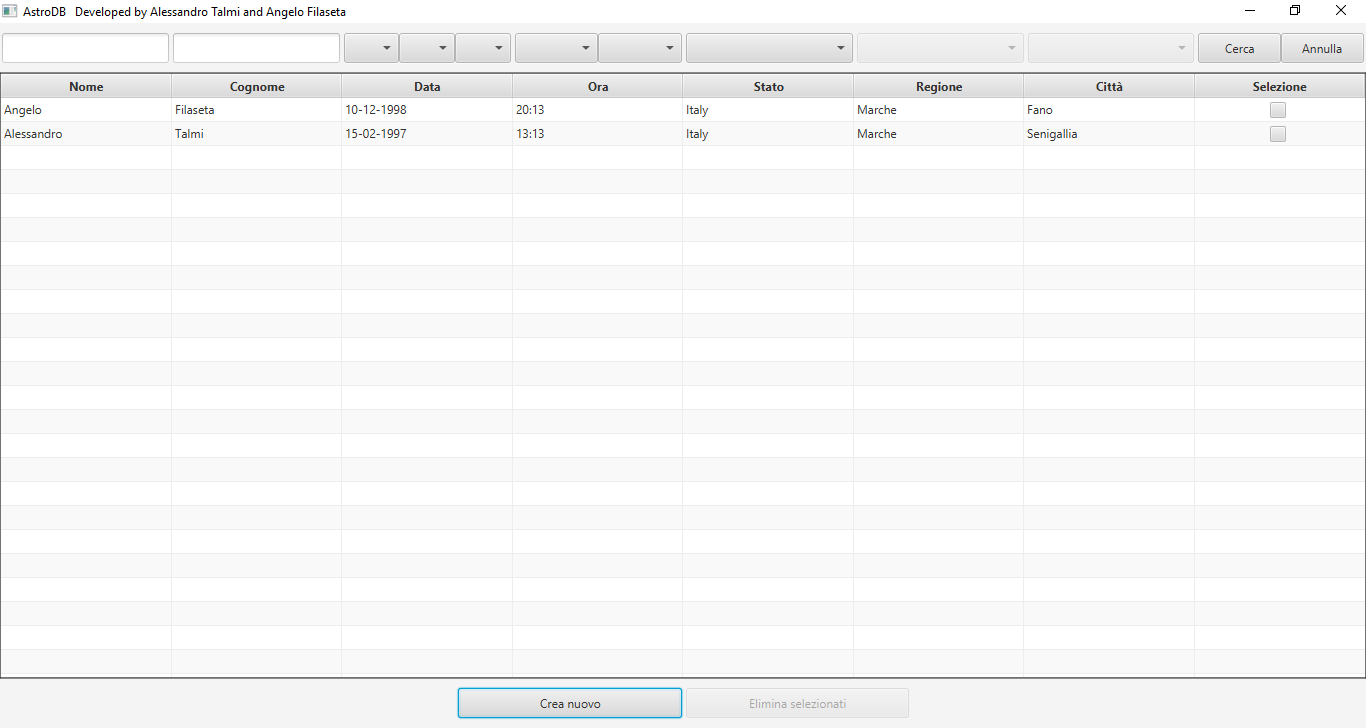
\includegraphics[width=\textwidth, height=0.35\textheight, keepaspectratio]{img/c5/MainView.png}
\caption{Schermata Principale}
\label{fig:mainview}
\end{figure}
La schermata principale visualizza tutti i record (persone) inseriti all’interno del DB.\newline
Al centro vengono mostrate le informazioni principali riguardanti l’anagrafica della persona. Per ottenere i dettagli astrologici sarà sufficiente un doppio click sulla persona d’interesse.\newline
In alto troviamo un filtro. Attraverso i campi presenti sarà possibile filtrare i record per ogni informazione componente l’anagrafica della persona. Sono presenti due bottoni:
\begin{itemize}
\item “Cerca”: applica i filtri inseriti;
\item “Annulla” elimina in un colpo solo tutti i filtri di ricerca.
\end{itemize}
In basso infine troviamo due bottoni:
\begin{itemize}
\item “Crea nuovo”: permette l’inserimento di un nuovo record;
\item “Elimina selezionati”: permette di eliminare i record selezionati attraverso la checkbox nella colonna “Selezione” (finché nessun record è selezionato il bottone sarà disabilitato).
\end{itemize}

\section{Dettagli di un Record}
Partendo dalla schermata principale ed effettuando un doppio click su un record si accede alla schermata dei dettagli.
\begin{figure}[H]
\centering
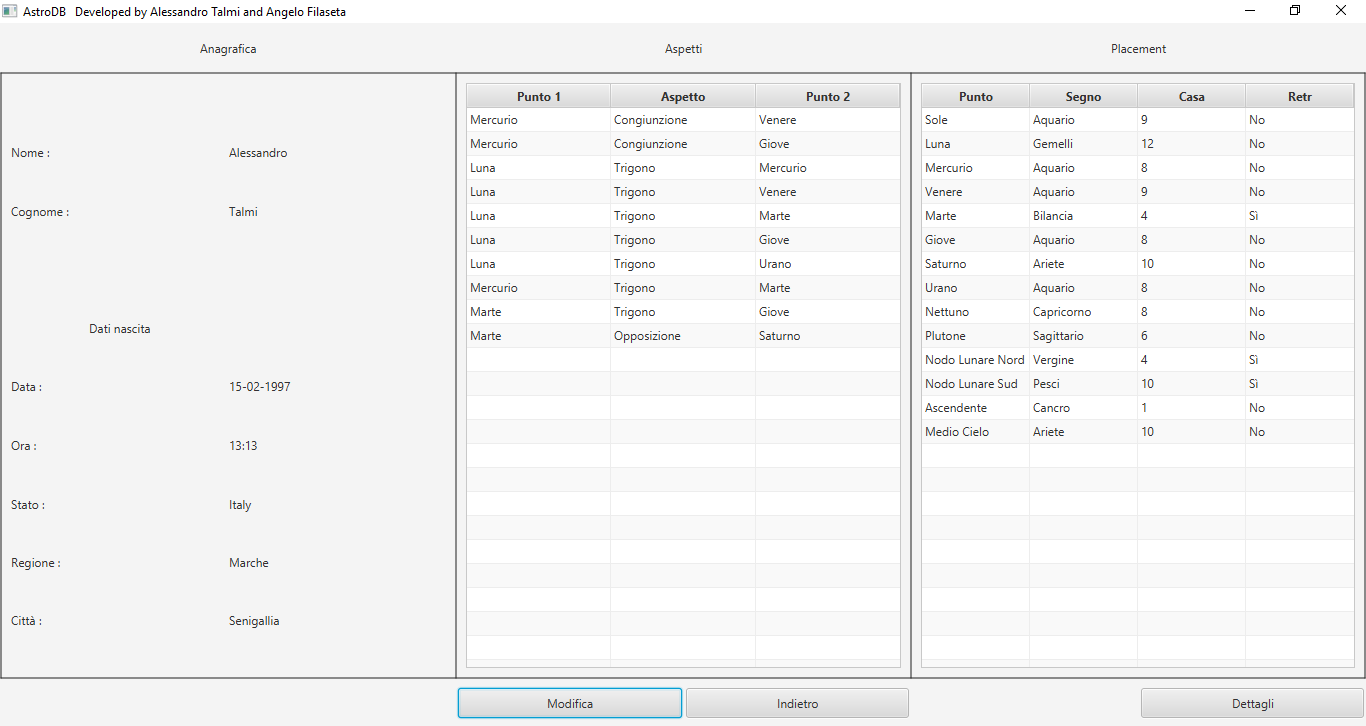
\includegraphics[width=\textwidth, height=0.35\textheight, keepaspectratio]{img/c5/PersonView.png}
\caption{Dettagli di un Record}
\label{fig:details}
\end{figure}

La schermata è divisa in tre sezioni:
\begin{enumerate}
  \item Anagrafica: In questa sezione troveremo tutte le informazioni riguardanti l’anagrafica di una persona (le stesse informazioni presenti nella schermata principale).
  \item Aspetti:
  Qui troveremo tutti gli Aspetti associati ad una persona. Attraverso un doppio click sarà possibile visualizzare un popup contenente ulteriori dettagli su quell’Aspetto
  \begin{figure}[H]
  \centering
  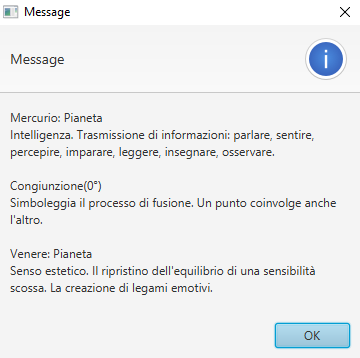
\includegraphics[width=\textwidth, height=0.35\textheight, keepaspectratio]{img/c5/AspectPopup.png}
  \caption{Dettagli dell'Aspetto}
  \label{fig:asppop}
  \end{figure}
  \item Placement:
  Analogamente alla sezione degli Aspetti qui troveremo tutti i Placement associati ad una persona e attraverso un doppio click potremo visualizzare ulteriori dettagli.
  \begin{figure}[H]
  \centering
  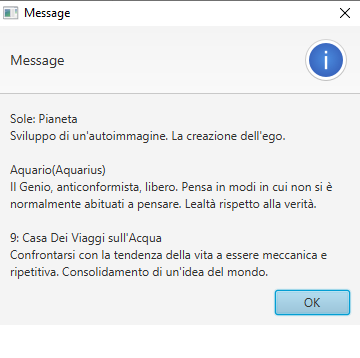
\includegraphics[width=\textwidth, height=0.35\textheight, keepaspectratio]{img/c5/PlacementPopup.png}
  \caption{Dettagli del Placement}
  \label{fig:placpop}
  \end{figure}
\end{enumerate}

In fondo troviamo 3 bottoni:
\begin{itemize}
  \item “Modifica”: permette di accedere alla schermata di modifica di un record;
  \item “Indietro”: permette di tornare alla schermata principale;
  \item “Dettagli”: permette di visualizzare un popup contenente le informazioni estrapolate dalle query dei dettagli astrologici;
  \begin{figure}[H]
  \centering
  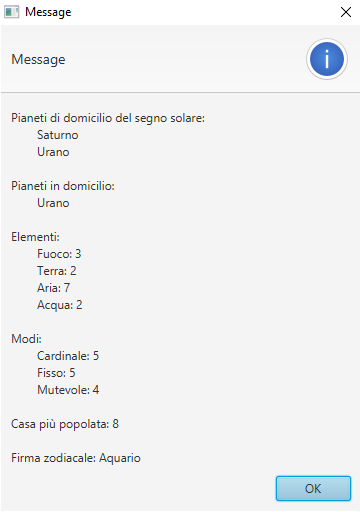
\includegraphics[width=\textwidth, height=0.35\textheight, keepaspectratio]{img/c5/DetailsPopup.png}
  \caption{Dettagli Astrologici}
  \label{fig:astrdet}
  \end{figure}
\end{itemize}


\section{Inserimento / Modifica}
La schermata di inserimento di un nuovo record coincide con la schermata di modifica di un record già esistente, con l’unica differenza che nel caso della modifica saranno già presenti le informazioni associate alla persona che si sta modificando.
\begin{figure}[H]
\centering
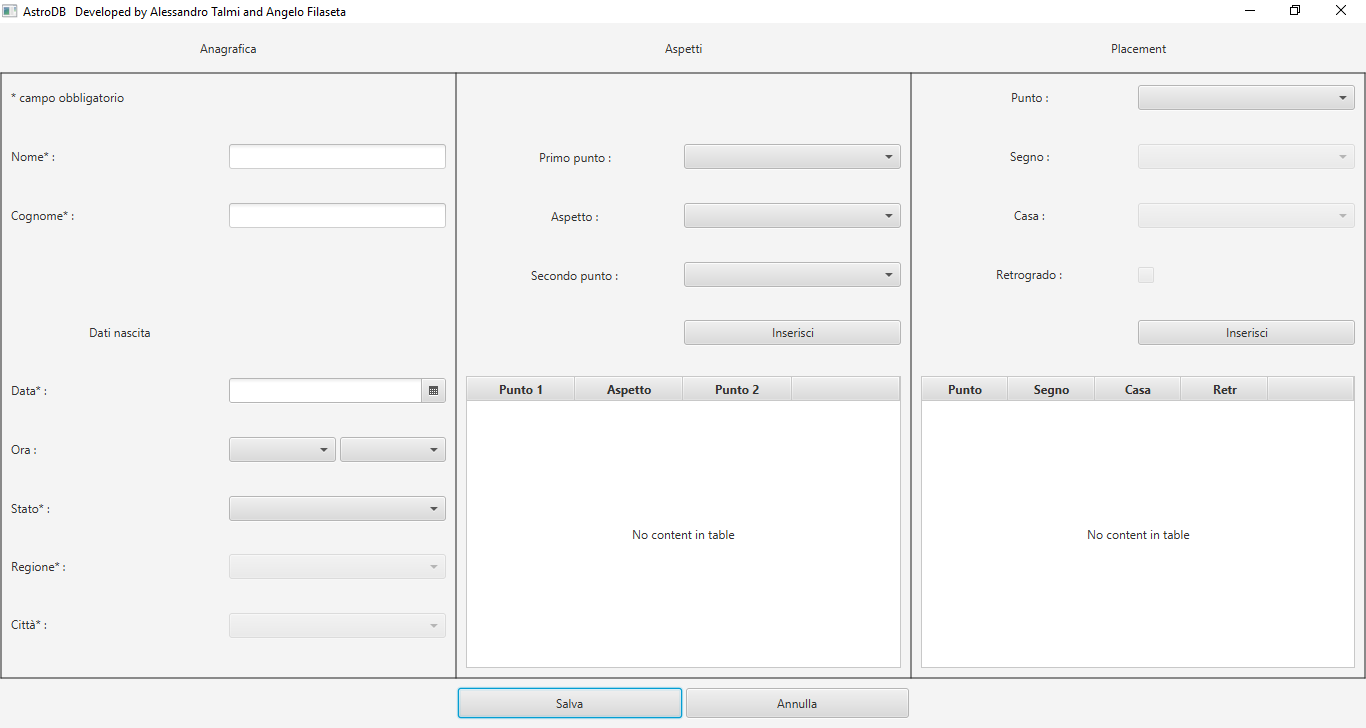
\includegraphics[width=\textwidth, height=0.35\textheight, keepaspectratio]{img/c5/InsertPerson.png}
\caption{Inserimento di una Persona}
\label{fig:inspers}
\end{figure}

\begin{figure}[H]
\centering
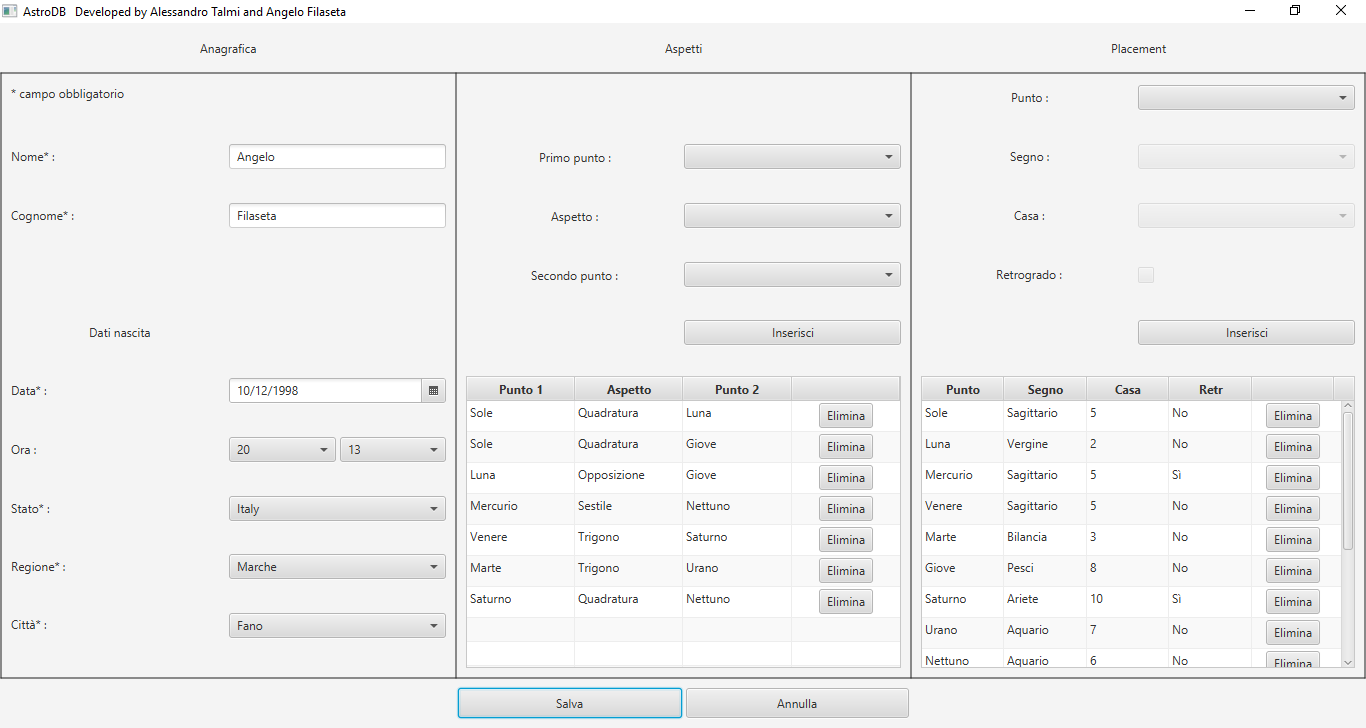
\includegraphics[width=\textwidth, height=0.35\textheight, keepaspectratio]{img/c5/ModifyPerson.png}
\caption{Modifica di una Persona}
\label{fig:modpers}
\end{figure}
La schermata è organizzata in modo totalmente analogo alla visualizzazione dei dettagli di un record:
\begin{itemize}
  \item Anagrafica:Qui andranno inserite le informazioni riguardanti l’anagrafica. I campi indicati con un asterisco sono obbligatori e l’inserimento/modifica non potrà essere salvato in assenza di esse;
\item Aspetti:
Qui andranno inseriti (attraverso il bottone “Inserisci”) gli Aspetti di una persona. Non sarà possibile inserire Aspetti in cui i due Punti coincidono (es: Luna – Sestile – Luna) né Aspetti contenenti una coppia di Punti già inseriti (es: se è stato inserito un Aspetto contenente Sole e Luna, non sarà possibile inserire né Sole – Luna né Luna – Sole). Analogamente alla vista dei dettagli attraverso un doppio click su un Aspetto verrà visualizzato un popup contenente ulteriori dettagli su quest’ultimo.
Il bottone “Elimina” di fianco ad ogni aspetto nella tabella permette appunto di eliminare quell’Aspetto;
\item Placement:
Qui andranno inseriti (attraverso il bottone “Inserisci”) i Placement di una persona. Non sarà possibile inserire Placement contenenti un Punto già presente all’interno di un placement inserito.
Anche qui il doppio click farà apparire un popup con le informazioni aggiuntive e il bottone “Elimina” eliminerà il placement selezionato.
\end{itemize}
In basso troviamo due bottoni:
\begin{itemize}
  \item “Salva”: se tutte le condizioni riguardanti i campi dell’anagrafica sono rispettate salva il record. Se si sta modificando un record si tornerà alla visualizzazione dei dettagli, altrimenti si tornerà alla schermata principale;
  \item “Annulla”: permette di tornare alla schermata di visualizzazione dei dettagli (o alla schermata principale) senza salvare le modifiche effettuate.
\end{itemize}
